\chapter{Metodoloxía seguida no desenvolvemento de Proxecto}

Os diferentes obxectivos do proxecto abordáronse seguindo a Metodoloxía SCRUM, adaptada a
un proxecto de un solo Developer.

Esta metodoloxía áxil tamén chamada melé pola súa inspiración no Rugby, permite un
desenvolvemento rápido en situacións de requisitos inestables. Apoiase no seu carácter 
iterativo e incremental, divindo o traballo a realizar en períodos de aproximadamente un mes
chamados Sprint's.

Para a realización deste traballo de fin de grao foi preciso adaptala, pois está pensada en 
principio para organizar equipos de entre 3 a 9 persoas (Team) mentres que neste caso só se contará 
cunha única persoa para desenvolver todo o proxecto. Por outro lado, o marco de 
traballo planifica reunións diarias (Daily Scrum), ao supoñer que todos os membros do equipo 
traballan unha xornada laboral enteira entre cada unha destas reunións, o cal tampouco se dá 
no caso deste proxecto, xa que a dedicación será de determinadas horas nos momentos dispoñibles.

\section{As metodoloxías áxiles}
    Escolleuse unha metodoloxía áxil como SCRUM para este proxecto xa que as metodoloxías áxiles en
    xeral son unha forma excepcional de minimizar os riscos asociados grazas ao seu carácter 
    iterativo (abordase por iteracións curtas de tempo) e incremental(as funcionalidades do proxecto
    crecen en cada iteración). Este carácter obriga a levar a cabo as fases de planificación, análise 
    de requisitos, deseño, codificación, revisión e documentación en cada Sprint, o cal se se 
    compara coas metodoloxías clásicas fai que tras un Sprint se poida axustar o seguinte en función
    de todo o aprendido, sen a necesidade dunha longa experiencia para poder planificar con 
    exactitude.
    
    Outra faceta importante das metodoloxías áxiles é a falta de documentación, isto está motivado 
    polos sucesivos cambios que se producen nestes proxectos por mor do seu caracter adaptativo, e 
    que serían moito mais custosos se ademais de modificar o propio software fose preciso modificar
    longas listas de documentación asociada. Por este motivo, neste sistema: a análise de requisitos 
    plasmarase como unha lista de tarefas que pasan ao Sprint Backlog, os diagramas de deseño só se 
    elaborarán para as partes mais críticas do sistema, no código evitaranse comentarios 
    innecesarios, e o plan de probas realizarase empregando unha folla excel en vez de un extenso 
    documento de texto.


\section{Persoas}

    Os tres papeis que se definen nesta metodoloxía \cite{la-guia-de-scrum} foron 
    adaptados do seguinte xeito:

    \subsection{ProductOwner}
        O papel de ProductOwner, que define os requisitos da aplicación estivo representado 
        polo director de proxecto Brais Cancela, que participou na creación do Anteproxecto.
        En certos momentos o señor Cancela tamén desempeñou a función de membro do equipo, 
        posto que é foi autor do algoritmo de análise de vídeo. 

    \subsection{ScrumMaster e Development Team}
        Ambos papeis leváronse a cabo polo autor, xa que carece de sentido definir ambas figuras
        nun equipo de unha soa persoa. De este xeito á par que se desenvolvía o proxecto, íase
        asegurando o cumprimento das regras de SCRUM.
    
\section{Reunións}
As reunións pola súa parte modifícanse do seguinte xeito:

    \subsection{Sprint Planning Meeting}
        Esta reunión mantén o mesmo formato que no SCRUM puro, xuntando ao autor co	ProductOwner 
        e concretando as tarefas do Product Backlog que se realizarán no seguinte Sprint, pasando
        por tanto a formar parte do Sprint Backlog.
    
    \subsection{Daily Scrum}
        Dado que o equipo de Desenvolvemento e o ScrumMaster están conformados pola mesma persoa
        e que o número de horas diarias adicadas é moito menos ao dunha xornada laboral, considerouse
        oportuno substituír esta reunión diaria por unha reunión dúas veces á semana (Martes e Xoves 
        pola tarde normalmente). Na que se mostrase ao ProductOwner o avance do proxecto.
    
    \subsection{Sprint Review}
        Esta reunión fusionase co Sprint Planning Meeting, xa que ao mesmo tempo valorase o traballo
        realizado no Sprint que remata e, en base a el, planificase a videira Iteración. 
    
    \subsection{Sprint Retrospective}
        Pola súa parte, esta reunión toma un carácter unipersoal, pasando a ser unha valoración do
        propio autor sobre as persoas, relaciones, procesos e ferramentas implicadas no último Sprint.
        Nela avalíase os elementos con éxito e os suxeitos a melloras, creando un plan para implementar
        estas melloras na Videira iteración.

\section{Control de Versións con GitHub}
    Os sistemas de control de versións permiten a xestión dos distintos cambios efectuados sobre
    un produto software ou sobre a súa configuración. Facilitando a administración das distintas
    versións do produto. 
    
    En concreto, GitHub é unha plataforma de desenvolvemento colaborativo que emprega o sistema de
    control de versións Git. Escolleuse empregar este sistema pola súa potencia e simplicidade, xa
    que proporciona libre acceso aos titores para comprobar o avance do proxecto, e a súa vez asegura
    que o código este sempre a bo recaudo.
    
    A páxina do proxecto é: \url{https://github.com/iago-suarez/ancoweb-TFG} 
    
\section{Integración Continua con Travis CI}

    A Integración Contínua (CI do ingles Continuous Integration) é un modelo informático que 
    consiste en facer integracións automáticas dun proxecto o mais a miúdo posible para así 
    poder detectar os posibles erros o antes posible, minimizando as súas posibles consecuencias.
    Outro factor importante é o feito de garantir que a versión subida ao repositorio segue a
    funcionar con independencia do entorno de desenvolvemento. Enténdense como pertencentes á 
    integración continua a compilación e a execución das probas de todo un proxecto.
    
    Travis CI é unha plataforma de integración continua para proxectos aloxados en GitHub, que 
    detecta automaticamente cando se produce un cambio no repositorio, e executa unha serie de pasos 
    definidos no ficheiro .travis.yml \ref{fig:travisYml}, que contén as accións a realizar 
    antes, durante e tras a as probas.
    
    Escolleuse Travis CI, pola súa integración con GitHub, pola súa potencia(permite executar 
    practicamente todo o que se pode executar nunha máquina local) e pola súa sinxela integración
    con outras ferramentas como Coveralls.
    
    \begin{figure}[!htp]
    \begin{center}
        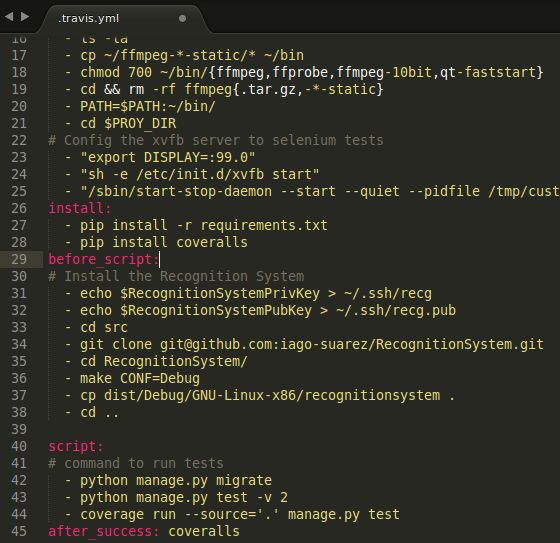
\includegraphics[scale=0.6]{figures/travisYml.png}
        \caption{Imaxe de parte do ficheiro .travis.yml}
    \label{fig:travisYml}
    \end{center}
    \end{figure}
    
    
\section{Control da cobertura con Coveralls}

\section{Xestión de Incidencias e Control de Proxecto con YouTrack}
    Co fin de levar a cabo un control das tarefas do Product Backlog e Sprint Backlog realizadas e 
    pendentes empregarase YouTrack como Sistema de Xestión de Incidencias (Issue Tracking System). 
    Un sistema de xestión de incidencias serve para xestionar as distintas incidencias (Tarefas 
    pendentes, Bug's, Problemas de usabilidade ou rendemento...) que poidan ter lugar nun entorno 
    como o proxecto web que nos ocupa. A estes efectos YouTrack mostrase como un completo sistema 
    de incidencias que permite a estimación e xestión de tempos, o emprego de comentarios para cada
    incidencia, buscas avanzadas, filtrado de incidencias, etc.
    
    Nótese que tamén se tiveron en conta outros sistemas de xestión de Incidencias como Redmine ou
    o sistema de xestión de incidencias integrado de GitHub, pero finalmente escolleuse YouTrack 
    pola súa coherencia coa filosofía áxil que se pode ver nos seus Paneis Áxiles, neles pódense
    xestionar todas as incidencias dun Sprint mediante o modelo Kanban, simplemente desprazando unha
    tarefa da columna de Tarefas Abertas á de Tarefas en Curso ou de esta última á de Tarefas 
    Solucionadas.
    
    \begin{figure}[htp]
    \begin{center}
        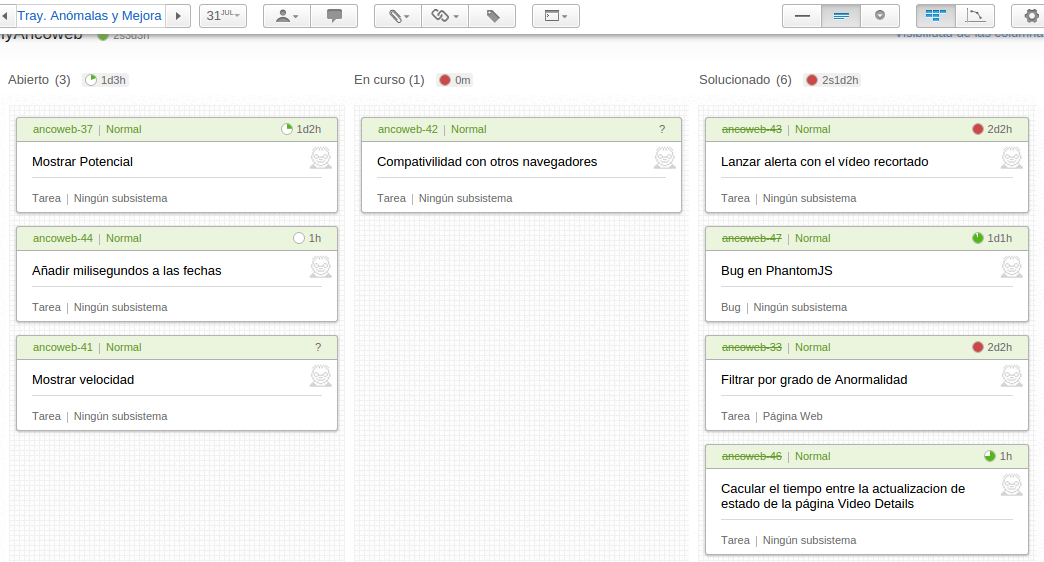
\includegraphics[scale=0.4]{figures/AgilePanel.png}
        \caption{Panel Áxil da ferramenta de xestión de incidencias YouTrack}
    \label{fig:AgilePanel}
    \end{center}
    \end{figure}
    
    
    

